\documentclass[1p]{elsarticle_modified}
%\bibliographystyle{elsarticle-num}

%\usepackage[colorlinks]{hyperref}
%\usepackage{abbrmath_seonhwa} %\Abb, \Ascr, \Acal ,\Abf, \Afrak
\usepackage{amsfonts}
\usepackage{amssymb}
\usepackage{amsmath}
\usepackage{amsthm}
\usepackage{scalefnt}
\usepackage{amsbsy}
\usepackage{kotex}
\usepackage{caption}
\usepackage{subfig}
\usepackage{color}
\usepackage{graphicx}
\usepackage{xcolor} %% white, black, red, green, blue, cyan, magenta, yellow
\usepackage{float}
\usepackage{setspace}
\usepackage{hyperref}

\usepackage{tikz}
\usetikzlibrary{arrows}

\usepackage{multirow}
\usepackage{array} % fixed length table
\usepackage{hhline}

%%%%%%%%%%%%%%%%%%%%%
\makeatletter
\renewcommand*\env@matrix[1][\arraystretch]{%
	\edef\arraystretch{#1}%
	\hskip -\arraycolsep
	\let\@ifnextchar\new@ifnextchar
	\array{*\c@MaxMatrixCols c}}
\makeatother %https://tex.stackexchange.com/questions/14071/how-can-i-increase-the-line-spacing-in-a-matrix
%%%%%%%%%%%%%%%

\usepackage[normalem]{ulem}

\newcommand{\msout}[1]{\ifmmode\text{\sout{\ensuremath{#1}}}\else\sout{#1}\fi}
%SOURCE: \msout is \stkout macro in https://tex.stackexchange.com/questions/20609/strikeout-in-math-mode

\newcommand{\cancel}[1]{
	\ifmmode
	{\color{red}\msout{#1}}
	\else
	{\color{red}\sout{#1}}
	\fi
}

\newcommand{\add}[1]{
	{\color{blue}\uwave{#1}}
}

\newcommand{\replace}[2]{
	\ifmmode
	{\color{red}\msout{#1}}{\color{blue}\uwave{#2}}
	\else
	{\color{red}\sout{#1}}{\color{blue}\uwave{#2}}
	\fi
}

\newcommand{\Sol}{\mathcal{S}} %segment
\newcommand{\D}{D} %diagram
\newcommand{\A}{\mathcal{A}} %arc


%%%%%%%%%%%%%%%%%%%%%%%%%%%%%5 test

\def\sl{\operatorname{\textup{SL}}(2,\Cbb)}
\def\psl{\operatorname{\textup{PSL}}(2,\Cbb)}
\def\quan{\mkern 1mu \triangleright \mkern 1mu}

\theoremstyle{definition}
\newtheorem{thm}{Theorem}[section]
\newtheorem{prop}[thm]{Proposition}
\newtheorem{lem}[thm]{Lemma}
\newtheorem{ques}[thm]{Question}
\newtheorem{cor}[thm]{Corollary}
\newtheorem{defn}[thm]{Definition}
\newtheorem{exam}[thm]{Example}
\newtheorem{rmk}[thm]{Remark}
\newtheorem{alg}[thm]{Algorithm}

\newcommand{\I}{\sqrt{-1}}
\begin{document}

%\begin{frontmatter}
%
%\title{Boundary parabolic representations of knots up to 8 crossings}
%
%%% Group authors per affiliation:
%\author{Yunhi Cho} 
%\address{Department of Mathematics, University of Seoul, Seoul, Korea}
%\ead{yhcho@uos.ac.kr}
%
%
%\author{Seonhwa Kim} %\fnref{s_kim}}
%\address{Center for Geometry and Physics, Institute for Basic Science, Pohang, 37673, Korea}
%\ead{ryeona17@ibs.re.kr}
%
%\author{Hyuk Kim}
%\address{Department of Mathematical Sciences, Seoul National University, Seoul 08826, Korea}
%\ead{hyukkim@snu.ac.kr}
%
%\author{Seokbeom Yoon}
%\address{Department of Mathematical Sciences, Seoul National University, Seoul, 08826,  Korea}
%\ead{sbyoon15@snu.ac.kr}
%
%\begin{abstract}
%We find all boundary parabolic representation of knots up to 8 crossings.
%
%\end{abstract}
%\begin{keyword}
%    \MSC[2010] 57M25 
%\end{keyword}
%
%\end{frontmatter}

%\linenumbers
%\tableofcontents
%
\newcommand\colored[1]{\textcolor{white}{\rule[-0.35ex]{0.8em}{1.4ex}}\kern-0.8em\color{red} #1}%
%\newcommand\colored[1]{\textcolor{white}{ #1}\kern-2.17ex	\textcolor{white}{ #1}\kern-1.81ex	\textcolor{white}{ #1}\kern-2.15ex\color{red}#1	}

{\Large $\underline{12n_{0099}~(K12n_{0099})}$}

\setlength{\tabcolsep}{10pt}
\renewcommand{\arraystretch}{1.6}
\vspace{1cm}\begin{tabular}{m{100pt}>{\centering\arraybackslash}m{274pt}}
\multirow{5}{120pt}{
	\centering
	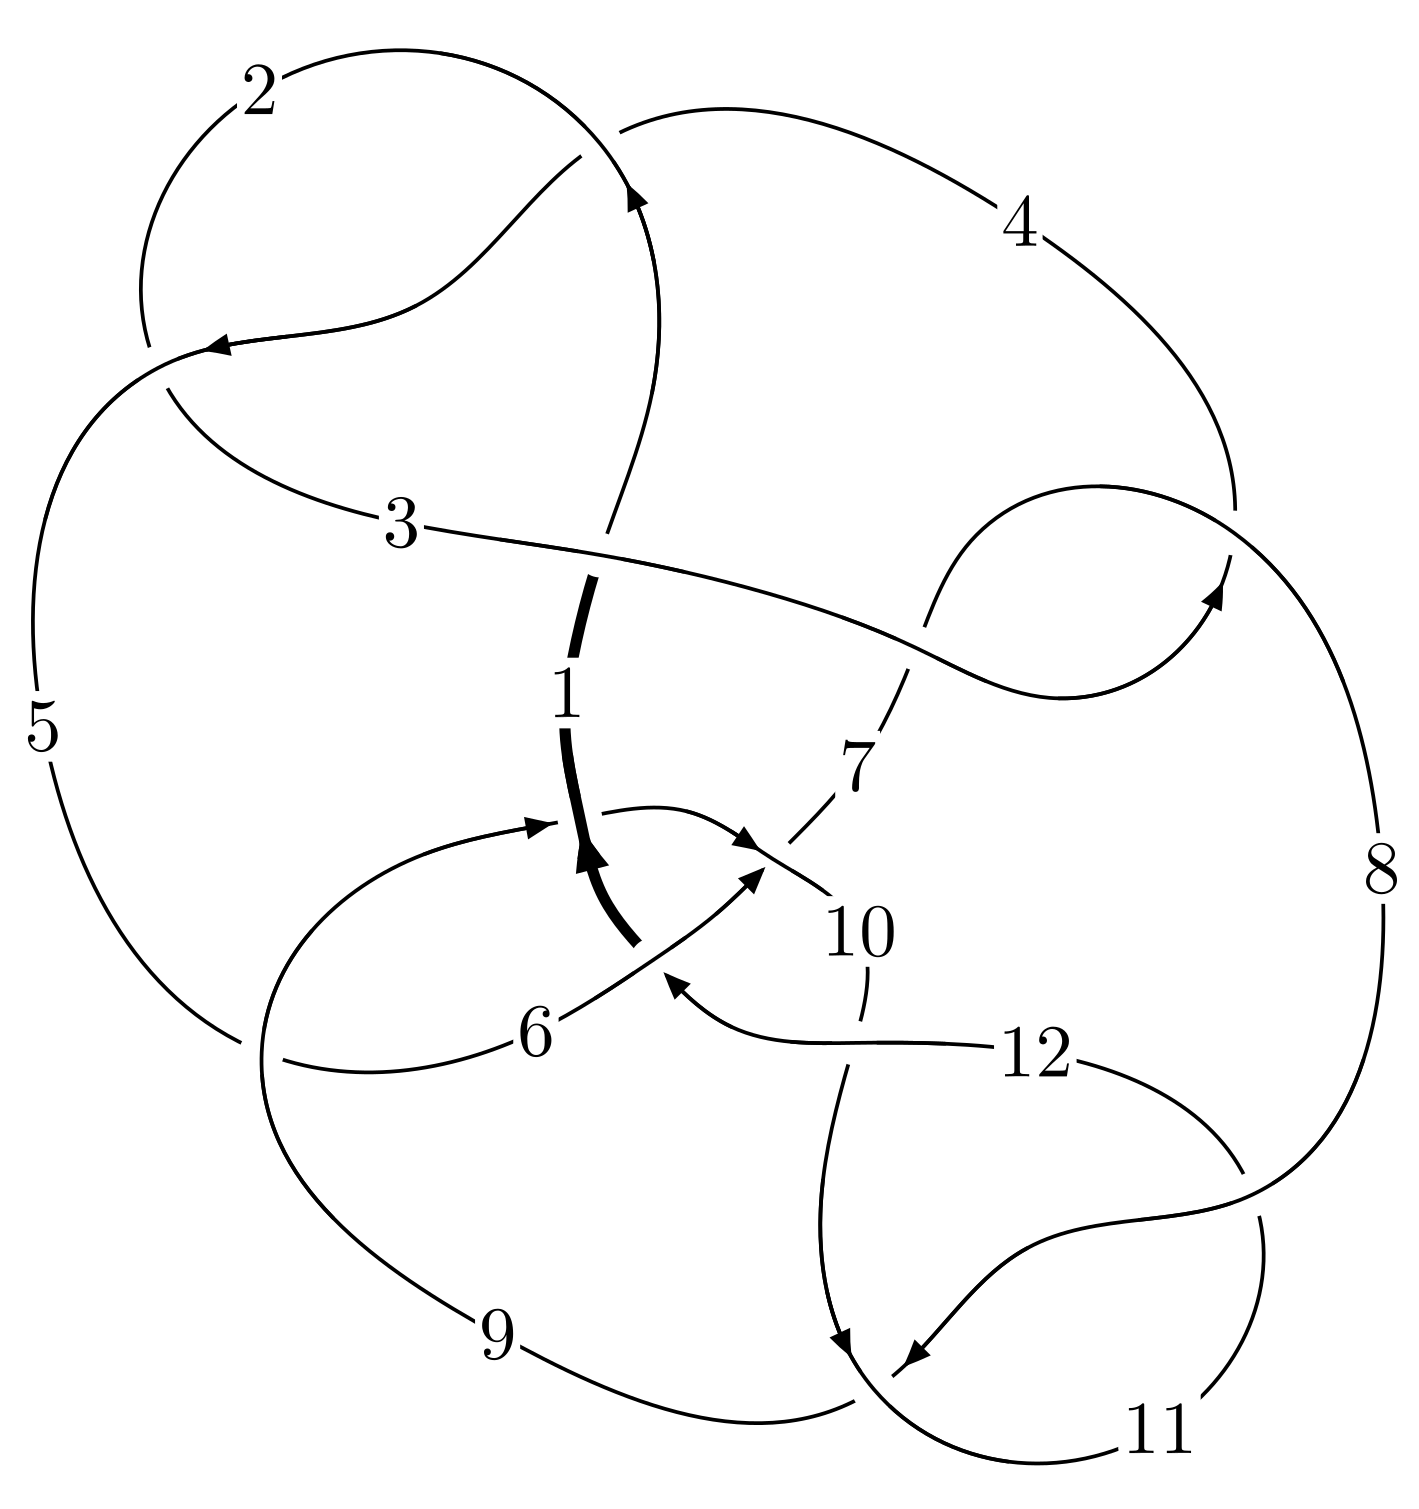
\includegraphics[width=112pt]{../../../GIT/diagram.site/Diagrams/png/2188_12n_0099.png}\\
\ \ \ A knot diagram\footnotemark}&
\allowdisplaybreaks
\textbf{Linearized knot diagam} \\
\cline{2-2}
 &
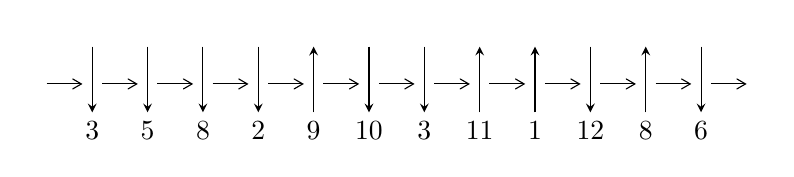
\begin{tikzpicture}[x=20pt, y=17pt]
	% nodes
	\node (C0) at (0, 0) {};
	\node (C1) at (1, 0) {};
	\node (C1U) at (1, +1) {};
	\node (C1D) at (1, -1) {3};

	\node (C2) at (2, 0) {};
	\node (C2U) at (2, +1) {};
	\node (C2D) at (2, -1) {5};

	\node (C3) at (3, 0) {};
	\node (C3U) at (3, +1) {};
	\node (C3D) at (3, -1) {8};

	\node (C4) at (4, 0) {};
	\node (C4U) at (4, +1) {};
	\node (C4D) at (4, -1) {2};

	\node (C5) at (5, 0) {};
	\node (C5U) at (5, +1) {};
	\node (C5D) at (5, -1) {9};

	\node (C6) at (6, 0) {};
	\node (C6U) at (6, +1) {};
	\node (C6D) at (6, -1) {10};

	\node (C7) at (7, 0) {};
	\node (C7U) at (7, +1) {};
	\node (C7D) at (7, -1) {3};

	\node (C8) at (8, 0) {};
	\node (C8U) at (8, +1) {};
	\node (C8D) at (8, -1) {11};

	\node (C9) at (9, 0) {};
	\node (C9U) at (9, +1) {};
	\node (C9D) at (9, -1) {1};

	\node (C10) at (10, 0) {};
	\node (C10U) at (10, +1) {};
	\node (C10D) at (10, -1) {12};

	\node (C11) at (11, 0) {};
	\node (C11U) at (11, +1) {};
	\node (C11D) at (11, -1) {8};

	\node (C12) at (12, 0) {};
	\node (C12U) at (12, +1) {};
	\node (C12D) at (12, -1) {6};
	\node (C13) at (13, 0) {};

	% arrows
	\draw[->,>={angle 60}]
	(C0) edge (C1) (C1) edge (C2) (C2) edge (C3) (C3) edge (C4) (C4) edge (C5) (C5) edge (C6) (C6) edge (C7) (C7) edge (C8) (C8) edge (C9) (C9) edge (C10) (C10) edge (C11) (C11) edge (C12) (C12) edge (C13) ;	\draw[->,>=stealth]
	(C1U) edge (C1D) (C2U) edge (C2D) (C3U) edge (C3D) (C4U) edge (C4D) (C5D) edge (C5U) (C6U) edge (C6D) (C7U) edge (C7D) (C8D) edge (C8U) (C9D) edge (C9U) (C10U) edge (C10D) (C11D) edge (C11U) (C12U) edge (C12D) ;
	\end{tikzpicture} \\
\hhline{~~} \\& 
\textbf{Solving Sequence} \\ \cline{2-2} 
 &
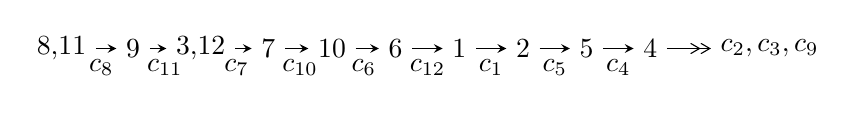
\begin{tikzpicture}[x=23pt, y=7pt]
	% node
	\node (A0) at (-1/8, 0) {8,11};
	\node (A1) at (1, 0) {9};
	\node (A2) at (33/16, 0) {3,12};
	\node (A3) at (25/8, 0) {7};
	\node (A4) at (33/8, 0) {10};
	\node (A5) at (41/8, 0) {6};
	\node (A6) at (49/8, 0) {1};
	\node (A7) at (57/8, 0) {2};
	\node (A8) at (65/8, 0) {5};
	\node (A9) at (73/8, 0) {4};
	\node (C1) at (1/2, -1) {$c_{8}$};
	\node (C2) at (3/2, -1) {$c_{11}$};
	\node (C3) at (21/8, -1) {$c_{7}$};
	\node (C4) at (29/8, -1) {$c_{10}$};
	\node (C5) at (37/8, -1) {$c_{6}$};
	\node (C6) at (45/8, -1) {$c_{12}$};
	\node (C7) at (53/8, -1) {$c_{1}$};
	\node (C8) at (61/8, -1) {$c_{5}$};
	\node (C9) at (69/8, -1) {$c_{4}$};
	\node (A10) at (11, 0) {$c_{2},c_{3},c_{9}$};

	% edge
	\draw[->,>=stealth]	
	(A0) edge (A1) (A1) edge (A2) (A2) edge (A3) (A3) edge (A4) (A4) edge (A5) (A5) edge (A6) (A6) edge (A7) (A7) edge (A8) (A8) edge (A9) ;
	\draw[->>,>={angle 60}]	
	(A9) edge (A10);
\end{tikzpicture} \\ 

\end{tabular} \\

\footnotetext{
The image of knot diagram is generated by the software ``\textbf{Draw programme}" developed by Andrew Bartholomew(\url{http://www.layer8.co.uk/maths/draw/index.htm\#Running-draw}), where we modified some parts for our purpose(\url{https://github.com/CATsTAILs/LinksPainter}).
}\phantom \\ \newline 
\centering \textbf{Ideals for irreducible components\footnotemark of $X_{\text{par}}$} 
 
\begin{align*}
I^u_{1}&=\langle 
-5.67717\times10^{122} u^{80}+2.40640\times10^{123} u^{79}+\cdots+1.36344\times10^{123} b-1.28567\times10^{122},\\
\phantom{I^u_{1}}&\phantom{= \langle  }-1.49380\times10^{122} u^{80}+9.63422\times10^{122} u^{79}+\cdots+6.81720\times10^{122} a-3.22718\times10^{124},\\
\phantom{I^u_{1}}&\phantom{= \langle  }u^{81}-4 u^{80}+\cdots+83 u+1\rangle \\
I^u_{2}&=\langle 
b,\;- u^3+a-2,\;u^4+u^2+u+1\rangle \\
I^u_{3}&=\langle 
b,\;- u^3+u^2+a-2 u+1,\;u^6- u^5+2 u^4-2 u^3+2 u^2-2 u+1\rangle \\
I^u_{4}&=\langle 
- a u+b+2 u,\;a^2+a u-3 a-3 u+2,\;u^2+u+1\rangle \\
\\
\end{align*}
\raggedright * 4 irreducible components of $\dim_{\mathbb{C}}=0$, with total 95 representations.\\
\footnotetext{All coefficients of polynomials are rational numbers. But the coefficients are sometimes approximated in decimal forms when there is not enough margin.}
\newpage
\renewcommand{\arraystretch}{1}
\centering \section*{I. $I^u_{1}= \langle -5.68\times10^{122} u^{80}+2.41\times10^{123} u^{79}+\cdots+1.36\times10^{123} b-1.29\times10^{122},\;-1.49\times10^{122} u^{80}+9.63\times10^{122} u^{79}+\cdots+6.82\times10^{122} a-3.23\times10^{124},\;u^{81}-4 u^{80}+\cdots+83 u+1 \rangle$}
\flushleft \textbf{(i) Arc colorings}\\
\begin{tabular}{m{7pt} m{180pt} m{7pt} m{180pt} }
\flushright $a_{8}=$&$\begin{pmatrix}1\\0\end{pmatrix}$ \\
\flushright $a_{11}=$&$\begin{pmatrix}0\\u\end{pmatrix}$ \\
\flushright $a_{9}=$&$\begin{pmatrix}1\\- u^2\end{pmatrix}$ \\
\flushright $a_{3}=$&$\begin{pmatrix}0.219123 u^{80}-1.41322 u^{79}+\cdots+157.415 u+47.3388\\0.416386 u^{80}-1.76495 u^{79}+\cdots-43.2149 u+0.0942957\end{pmatrix}$ \\
\flushright $a_{12}=$&$\begin{pmatrix}u\\u\end{pmatrix}$ \\
\flushright $a_{7}=$&$\begin{pmatrix}-0.327866 u^{80}+1.87240 u^{79}+\cdots-62.8797 u-27.5857\\-0.435511 u^{80}+1.87462 u^{79}+\cdots+47.9628 u+0.199503\end{pmatrix}$ \\
\flushright $a_{10}=$&$\begin{pmatrix}u^3\\u^3+u\end{pmatrix}$ \\
\flushright $a_{6}=$&$\begin{pmatrix}-0.236666 u^{80}+1.65002 u^{79}+\cdots-61.3415 u-27.5686\\-0.457531 u^{80}+2.08795 u^{79}+\cdots+57.2670 u+0.314050\end{pmatrix}$ \\
\flushright $a_{1}=$&$\begin{pmatrix}0.253925 u^{80}-0.469551 u^{79}+\cdots+57.0053 u+9.60025\\-0.376132 u^{80}+1.67454 u^{79}+\cdots+43.3245 u+0.630057\end{pmatrix}$ \\
\flushright $a_{2}=$&$\begin{pmatrix}0.0290630 u^{80}-0.406433 u^{79}+\cdots+115.361 u+29.5970\\0.334532 u^{80}-1.24445 u^{79}+\cdots-23.7001 u+0.0863807\end{pmatrix}$ \\
\flushright $a_{5}=$&$\begin{pmatrix}-0.567784 u^{80}+2.57406 u^{79}+\cdots-60.4666 u-27.1793\\-0.334532 u^{80}+1.24445 u^{79}+\cdots+23.7001 u-0.0863807\end{pmatrix}$ \\
\flushright $a_{4}=$&$\begin{pmatrix}0.197263 u^{80}-0.351727 u^{79}+\cdots-200.629 u-47.2445\\-0.416386 u^{80}+1.76495 u^{79}+\cdots+43.2149 u-0.0942957\end{pmatrix}$\\&\end{tabular}
\flushleft \textbf{(ii) Obstruction class $= -1$}\\~\\
\flushleft \textbf{(iii) Cusp Shapes $= 0.523679 u^{80}-1.64827 u^{79}+\cdots+61.1096 u-9.44591$}\\~\\
\newpage\renewcommand{\arraystretch}{1}
\flushleft \textbf{(iv) u-Polynomials at the component}\newline \\
\begin{tabular}{m{50pt}|m{274pt}}
Crossings & \hspace{64pt}u-Polynomials at each crossing \\
\hline $$\begin{aligned}c_{1}\end{aligned}$$&$\begin{aligned}
&u^{81}+33 u^{80}+\cdots+130 u+1
\end{aligned}$\\
\hline $$\begin{aligned}c_{2},c_{4}\end{aligned}$$&$\begin{aligned}
&u^{81}-13 u^{80}+\cdots-12 u+1
\end{aligned}$\\
\hline $$\begin{aligned}c_{3},c_{7}\end{aligned}$$&$\begin{aligned}
&u^{81}-3 u^{80}+\cdots+1024 u+1024
\end{aligned}$\\
\hline $$\begin{aligned}c_{5}\end{aligned}$$&$\begin{aligned}
&u^{81}+u^{80}+\cdots+8905262 u+2124511
\end{aligned}$\\
\hline $$\begin{aligned}c_{6}\end{aligned}$$&$\begin{aligned}
&u^{81}+5 u^{80}+\cdots-47488 u+22208
\end{aligned}$\\
\hline $$\begin{aligned}c_{8},c_{11}\end{aligned}$$&$\begin{aligned}
&u^{81}+4 u^{80}+\cdots+83 u-1
\end{aligned}$\\
\hline $$\begin{aligned}c_{9}\end{aligned}$$&$\begin{aligned}
&u^{81}+8 u^{80}+\cdots+256 u+16
\end{aligned}$\\
\hline $$\begin{aligned}c_{10}\end{aligned}$$&$\begin{aligned}
&u^{81}+30 u^{80}+\cdots+6303 u-1
\end{aligned}$\\
\hline $$\begin{aligned}c_{12}\end{aligned}$$&$\begin{aligned}
&u^{81}-4 u^{80}+\cdots-5 u+1
\end{aligned}$\\
\hline
\end{tabular}\\~\\
\newpage\renewcommand{\arraystretch}{1}
\flushleft \textbf{(v) Riley Polynomials at the component}\newline \\
\begin{tabular}{m{50pt}|m{274pt}}
Crossings & \hspace{64pt}Riley Polynomials at each crossing \\
\hline $$\begin{aligned}c_{1}\end{aligned}$$&$\begin{aligned}
&y^{81}+43 y^{80}+\cdots+5274 y-1
\end{aligned}$\\
\hline $$\begin{aligned}c_{2},c_{4}\end{aligned}$$&$\begin{aligned}
&y^{81}-33 y^{80}+\cdots+130 y-1
\end{aligned}$\\
\hline $$\begin{aligned}c_{3},c_{7}\end{aligned}$$&$\begin{aligned}
&y^{81}+57 y^{80}+\cdots-27787264 y-1048576
\end{aligned}$\\
\hline $$\begin{aligned}c_{5}\end{aligned}$$&$\begin{aligned}
&y^{81}+47 y^{80}+\cdots+59668081079090 y-4513546989121
\end{aligned}$\\
\hline $$\begin{aligned}c_{6}\end{aligned}$$&$\begin{aligned}
&y^{81}+103 y^{80}+\cdots-19451522048 y-493195264
\end{aligned}$\\
\hline $$\begin{aligned}c_{8},c_{11}\end{aligned}$$&$\begin{aligned}
&y^{81}+30 y^{80}+\cdots+6303 y-1
\end{aligned}$\\
\hline $$\begin{aligned}c_{9}\end{aligned}$$&$\begin{aligned}
&y^{81}-20 y^{80}+\cdots-1152 y-256
\end{aligned}$\\
\hline $$\begin{aligned}c_{10}\end{aligned}$$&$\begin{aligned}
&y^{81}+46 y^{80}+\cdots+39786411 y-1
\end{aligned}$\\
\hline $$\begin{aligned}c_{12}\end{aligned}$$&$\begin{aligned}
&y^{81}-6 y^{80}+\cdots+11 y-1
\end{aligned}$\\
\hline
\end{tabular}\\~\\
\newpage\flushleft \textbf{(vi) Complex Volumes and Cusp Shapes}
$$\begin{array}{c|c|c}  
\text{Solutions to }I^u_{1}& \I (\text{vol} + \sqrt{-1}CS) & \text{Cusp shape}\\
 \hline 
\begin{aligned}
u &= -0.505398 + 0.861438 I \\
a &= -4.37384 - 2.52183 I \\
b &= \phantom{-}0.603292 - 0.010555 I\end{aligned}
 & -1.02453 - 2.05291 I & -171.972 + 28.532 I \\ \hline\begin{aligned}
u &= -0.505398 - 0.861438 I \\
a &= -4.37384 + 2.52183 I \\
b &= \phantom{-}0.603292 + 0.010555 I\end{aligned}
 & -1.02453 + 2.05291 I & -171.972 - 28.532 I \\ \hline\begin{aligned}
u &= -0.009112 + 1.005390 I \\
a &= -0.308654 + 0.203514 I \\
b &= -0.336499 - 0.810387 I\end{aligned}
 & -4.60609 - 1.52975 I & \phantom{-0.000000 } 0 \\ \hline\begin{aligned}
u &= -0.009112 - 1.005390 I \\
a &= -0.308654 - 0.203514 I \\
b &= -0.336499 + 0.810387 I\end{aligned}
 & -4.60609 + 1.52975 I & \phantom{-0.000000 } 0 \\ \hline\begin{aligned}
u &= \phantom{-}0.742803 + 0.679982 I \\
a &= -0.167793 + 0.282223 I \\
b &= \phantom{-}0.67879 + 1.59644 I\end{aligned}
 & \phantom{-}6.21314 - 4.26930 I & \phantom{-0.000000 } 0 \\ \hline\begin{aligned}
u &= \phantom{-}0.742803 - 0.679982 I \\
a &= -0.167793 - 0.282223 I \\
b &= \phantom{-}0.67879 - 1.59644 I\end{aligned}
 & \phantom{-}6.21314 + 4.26930 I & \phantom{-0.000000 } 0 \\ \hline\begin{aligned}
u &= \phantom{-}0.724035 + 0.675293 I \\
a &= \phantom{-}1.163810 + 0.739644 I \\
b &= \phantom{-}0.239752 - 1.287670 I\end{aligned}
 & \phantom{-}0.58736 - 1.68614 I & \phantom{-0.000000 } 0 \\ \hline\begin{aligned}
u &= \phantom{-}0.724035 - 0.675293 I \\
a &= \phantom{-}1.163810 - 0.739644 I \\
b &= \phantom{-}0.239752 + 1.287670 I\end{aligned}
 & \phantom{-}0.58736 + 1.68614 I & \phantom{-0.000000 } 0 \\ \hline\begin{aligned}
u &= -0.264835 + 0.948397 I \\
a &= -0.02548 - 2.76624 I \\
b &= \phantom{-}0.086690 - 1.153850 I\end{aligned}
 & \phantom{-}1.73887 + 0.56914 I & \phantom{-0.000000 } 0 \\ \hline\begin{aligned}
u &= -0.264835 - 0.948397 I \\
a &= -0.02548 + 2.76624 I \\
b &= \phantom{-}0.086690 + 1.153850 I\end{aligned}
 & \phantom{-}1.73887 - 0.56914 I & \phantom{-0.000000 } 0\\
 \hline 
 \end{array}$$\newpage$$\begin{array}{c|c|c}  
\text{Solutions to }I^u_{1}& \I (\text{vol} + \sqrt{-1}CS) & \text{Cusp shape}\\
 \hline 
\begin{aligned}
u &= \phantom{-}0.479721 + 0.852602 I \\
a &= -1.22325 - 1.39529 I \\
b &= -1.59287 + 0.05128 I\end{aligned}
 & -8.92096 + 1.95711 I & -29.9268 + 41.7453 I \\ \hline\begin{aligned}
u &= \phantom{-}0.479721 - 0.852602 I \\
a &= -1.22325 + 1.39529 I \\
b &= -1.59287 - 0.05128 I\end{aligned}
 & -8.92096 - 1.95711 I & -29.9268 - 41.7453 I \\ \hline\begin{aligned}
u &= -0.615664 + 0.829871 I \\
a &= -1.37738 + 1.51974 I \\
b &= \phantom{-}0.154661 - 1.382630 I\end{aligned}
 & \phantom{-}3.68961 + 0.58365 I & \phantom{-0.000000 } 0 \\ \hline\begin{aligned}
u &= -0.615664 - 0.829871 I \\
a &= -1.37738 - 1.51974 I \\
b &= \phantom{-}0.154661 + 1.382630 I\end{aligned}
 & \phantom{-}3.68961 - 0.58365 I & \phantom{-0.000000 } 0 \\ \hline\begin{aligned}
u &= \phantom{-}0.825094 + 0.624144 I \\
a &= -0.916453 - 0.626602 I \\
b &= -1.357180 + 0.050552 I\end{aligned}
 & \phantom{-}2.74432 - 4.49163 I & \phantom{-0.000000 } 0 \\ \hline\begin{aligned}
u &= \phantom{-}0.825094 - 0.624144 I \\
a &= -0.916453 + 0.626602 I \\
b &= -1.357180 - 0.050552 I\end{aligned}
 & \phantom{-}2.74432 + 4.49163 I & \phantom{-0.000000 } 0 \\ \hline\begin{aligned}
u &= -0.524882 + 0.802233 I \\
a &= \phantom{-}4.37321 + 0.45617 I \\
b &= \phantom{-}0.458462 + 0.233945 I\end{aligned}
 & -1.11518 - 1.63608 I & -22.5154 + 16.4209 I \\ \hline\begin{aligned}
u &= -0.524882 - 0.802233 I \\
a &= \phantom{-}4.37321 - 0.45617 I \\
b &= \phantom{-}0.458462 - 0.233945 I\end{aligned}
 & -1.11518 + 1.63608 I & -22.5154 - 16.4209 I \\ \hline\begin{aligned}
u &= \phantom{-}0.703049 + 0.783366 I \\
a &= \phantom{-}0.83771 + 1.13988 I \\
b &= \phantom{-}1.42270 + 0.44570 I\end{aligned}
 & \phantom{-}1.96531 + 1.49483 I & \phantom{-0.000000 } 0 \\ \hline\begin{aligned}
u &= \phantom{-}0.703049 - 0.783366 I \\
a &= \phantom{-}0.83771 - 1.13988 I \\
b &= \phantom{-}1.42270 - 0.44570 I\end{aligned}
 & \phantom{-}1.96531 - 1.49483 I & \phantom{-0.000000 } 0\\
 \hline 
 \end{array}$$\newpage$$\begin{array}{c|c|c}  
\text{Solutions to }I^u_{1}& \I (\text{vol} + \sqrt{-1}CS) & \text{Cusp shape}\\
 \hline 
\begin{aligned}
u &= -0.026493 + 0.936757 I \\
a &= \phantom{-}0.59780 + 2.29454 I \\
b &= \phantom{-}0.439042 + 1.154740 I\end{aligned}
 & \phantom{-}0.95414 - 4.42889 I & -4.00000 + 4.19606 I \\ \hline\begin{aligned}
u &= -0.026493 - 0.936757 I \\
a &= \phantom{-}0.59780 - 2.29454 I \\
b &= \phantom{-}0.439042 - 1.154740 I\end{aligned}
 & \phantom{-}0.95414 + 4.42889 I & -4.00000 - 4.19606 I \\ \hline\begin{aligned}
u &= -0.671407 + 0.627762 I \\
a &= -0.913409 - 0.028748 I \\
b &= -0.412488 + 0.213180 I\end{aligned}
 & \phantom{-}1.15026 - 1.50439 I & \phantom{-}2.46877 + 2.61626 I \\ \hline\begin{aligned}
u &= -0.671407 - 0.627762 I \\
a &= -0.913409 + 0.028748 I \\
b &= -0.412488 - 0.213180 I\end{aligned}
 & \phantom{-}1.15026 + 1.50439 I & \phantom{-}2.46877 - 2.61626 I \\ \hline\begin{aligned}
u &= -0.599484 + 0.904512 I \\
a &= \phantom{-}2.63171 - 1.35351 I \\
b &= \phantom{-}0.277078 + 1.371800 I\end{aligned}
 & \phantom{-}3.45045 - 5.35632 I & \phantom{-0.000000 } 0 \\ \hline\begin{aligned}
u &= -0.599484 - 0.904512 I \\
a &= \phantom{-}2.63171 + 1.35351 I \\
b &= \phantom{-}0.277078 - 1.371800 I\end{aligned}
 & \phantom{-}3.45045 + 5.35632 I & \phantom{-0.000000 } 0 \\ \hline\begin{aligned}
u &= -0.561505 + 0.944951 I \\
a &= \phantom{-}1.70785 + 3.15850 I \\
b &= \phantom{-}0.110600 - 0.423339 I\end{aligned}
 & -1.63060 - 2.73282 I & \phantom{-0.000000 } 0 \\ \hline\begin{aligned}
u &= -0.561505 - 0.944951 I \\
a &= \phantom{-}1.70785 - 3.15850 I \\
b &= \phantom{-}0.110600 + 0.423339 I\end{aligned}
 & -1.63060 + 2.73282 I & \phantom{-0.000000 } 0 \\ \hline\begin{aligned}
u &= -0.455620 + 1.013820 I \\
a &= -0.238189 + 0.544842 I \\
b &= \phantom{-}0.029747 + 0.351694 I\end{aligned}
 & -0.39491 - 2.82152 I & \phantom{-0.000000 } 0 \\ \hline\begin{aligned}
u &= -0.455620 - 1.013820 I \\
a &= -0.238189 - 0.544842 I \\
b &= \phantom{-}0.029747 - 0.351694 I\end{aligned}
 & -0.39491 + 2.82152 I & \phantom{-0.000000 } 0\\
 \hline 
 \end{array}$$\newpage$$\begin{array}{c|c|c}  
\text{Solutions to }I^u_{1}& \I (\text{vol} + \sqrt{-1}CS) & \text{Cusp shape}\\
 \hline 
\begin{aligned}
u &= \phantom{-}0.761415 + 0.820530 I \\
a &= \phantom{-}0.531324 - 0.454947 I \\
b &= -0.42765 - 1.74880 I\end{aligned}
 & \phantom{-}8.06491 + 2.92024 I & \phantom{-0.000000 } 0 \\ \hline\begin{aligned}
u &= \phantom{-}0.761415 - 0.820530 I \\
a &= \phantom{-}0.531324 + 0.454947 I \\
b &= -0.42765 + 1.74880 I\end{aligned}
 & \phantom{-}8.06491 - 2.92024 I & \phantom{-0.000000 } 0 \\ \hline\begin{aligned}
u &= -0.108997 + 1.122070 I \\
a &= -2.39634 - 0.23797 I \\
b &= -0.890661 + 0.321140 I\end{aligned}
 & -3.72961 - 3.73093 I & \phantom{-0.000000 } 0 \\ \hline\begin{aligned}
u &= -0.108997 - 1.122070 I \\
a &= -2.39634 + 0.23797 I \\
b &= -0.890661 - 0.321140 I\end{aligned}
 & -3.72961 + 3.73093 I & \phantom{-0.000000 } 0 \\ \hline\begin{aligned}
u &= \phantom{-}0.997287 + 0.541891 I \\
a &= -0.369368 - 0.079618 I \\
b &= -0.66734 - 1.50573 I\end{aligned}
 & \phantom{-}7.29123 - 11.70270 I & \phantom{-0.000000 } 0 \\ \hline\begin{aligned}
u &= \phantom{-}0.997287 - 0.541891 I \\
a &= -0.369368 + 0.079618 I \\
b &= -0.66734 + 1.50573 I\end{aligned}
 & \phantom{-}7.29123 + 11.70270 I & \phantom{-0.000000 } 0 \\ \hline\begin{aligned}
u &= \phantom{-}0.959008 + 0.624962 I \\
a &= -0.148070 + 0.092204 I \\
b &= \phantom{-}0.36850 + 1.64315 I\end{aligned}
 & \phantom{-}9.10043 - 4.86820 I & \phantom{-0.000000 } 0 \\ \hline\begin{aligned}
u &= \phantom{-}0.959008 - 0.624962 I \\
a &= -0.148070 - 0.092204 I \\
b &= \phantom{-}0.36850 - 1.64315 I\end{aligned}
 & \phantom{-}9.10043 + 4.86820 I & \phantom{-0.000000 } 0 \\ \hline\begin{aligned}
u &= \phantom{-}0.682699 + 0.926132 I \\
a &= \phantom{-}1.43843 + 0.92415 I \\
b &= \phantom{-}1.54169 - 0.19466 I\end{aligned}
 & \phantom{-}1.52644 + 3.83350 I & \phantom{-0.000000 } 0 \\ \hline\begin{aligned}
u &= \phantom{-}0.682699 - 0.926132 I \\
a &= \phantom{-}1.43843 - 0.92415 I \\
b &= \phantom{-}1.54169 + 0.19466 I\end{aligned}
 & \phantom{-}1.52644 - 3.83350 I & \phantom{-0.000000 } 0\\
 \hline 
 \end{array}$$\newpage$$\begin{array}{c|c|c}  
\text{Solutions to }I^u_{1}& \I (\text{vol} + \sqrt{-1}CS) & \text{Cusp shape}\\
 \hline 
\begin{aligned}
u &= \phantom{-}0.745953 + 0.906662 I \\
a &= -1.80870 - 0.05187 I \\
b &= -0.63390 + 1.61836 I\end{aligned}
 & \phantom{-}7.80552 + 2.77364 I & \phantom{-0.000000 } 0 \\ \hline\begin{aligned}
u &= \phantom{-}0.745953 - 0.906662 I \\
a &= -1.80870 + 0.05187 I \\
b &= -0.63390 - 1.61836 I\end{aligned}
 & \phantom{-}7.80552 - 2.77364 I & \phantom{-0.000000 } 0 \\ \hline\begin{aligned}
u &= -0.714581 + 0.401247 I \\
a &= -1.165920 - 0.348917 I \\
b &= -0.616988 - 0.161976 I\end{aligned}
 & \phantom{-}1.29375 - 1.45245 I & \phantom{-}3.62930 + 4.86424 I \\ \hline\begin{aligned}
u &= -0.714581 - 0.401247 I \\
a &= -1.165920 + 0.348917 I \\
b &= -0.616988 + 0.161976 I\end{aligned}
 & \phantom{-}1.29375 + 1.45245 I & \phantom{-}3.62930 - 4.86424 I \\ \hline\begin{aligned}
u &= \phantom{-}0.062348 + 0.798476 I \\
a &= \phantom{-}1.53880 + 1.10941 I \\
b &= \phantom{-}0.880183 - 0.328930 I\end{aligned}
 & -2.15630 + 0.07606 I & -8.00350 + 0.07144 I \\ \hline\begin{aligned}
u &= \phantom{-}0.062348 - 0.798476 I \\
a &= \phantom{-}1.53880 - 1.10941 I \\
b &= \phantom{-}0.880183 + 0.328930 I\end{aligned}
 & -2.15630 - 0.07606 I & -8.00350 - 0.07144 I \\ \hline\begin{aligned}
u &= \phantom{-}0.675941 + 0.993873 I \\
a &= -0.976588 - 0.077747 I \\
b &= \phantom{-}0.00539 + 1.42943 I\end{aligned}
 & -0.36837 + 7.06216 I & \phantom{-0.000000 } 0 \\ \hline\begin{aligned}
u &= \phantom{-}0.675941 - 0.993873 I \\
a &= -0.976588 + 0.077747 I \\
b &= \phantom{-}0.00539 - 1.42943 I\end{aligned}
 & -0.36837 - 7.06216 I & \phantom{-0.000000 } 0 \\ \hline\begin{aligned}
u &= \phantom{-}0.680506 + 0.995566 I \\
a &= \phantom{-}2.16987 + 0.15146 I \\
b &= \phantom{-}0.83647 - 1.48482 I\end{aligned}
 & \phantom{-}5.25967 + 9.70670 I & \phantom{-0.000000 } 0 \\ \hline\begin{aligned}
u &= \phantom{-}0.680506 - 0.995566 I \\
a &= \phantom{-}2.16987 - 0.15146 I \\
b &= \phantom{-}0.83647 + 1.48482 I\end{aligned}
 & \phantom{-}5.25967 - 9.70670 I & \phantom{-0.000000 } 0\\
 \hline 
 \end{array}$$\newpage$$\begin{array}{c|c|c}  
\text{Solutions to }I^u_{1}& \I (\text{vol} + \sqrt{-1}CS) & \text{Cusp shape}\\
 \hline 
\begin{aligned}
u &= \phantom{-}0.753433 + 0.220803 I \\
a &= -0.235608 + 0.164102 I \\
b &= \phantom{-}0.020461 + 0.617454 I\end{aligned}
 & -1.20619 - 3.00339 I & \phantom{-}2.21341 + 3.98452 I \\ \hline\begin{aligned}
u &= \phantom{-}0.753433 - 0.220803 I \\
a &= -0.235608 - 0.164102 I \\
b &= \phantom{-}0.020461 - 0.617454 I\end{aligned}
 & -1.20619 + 3.00339 I & \phantom{-}2.21341 - 3.98452 I \\ \hline\begin{aligned}
u &= \phantom{-}0.292757 + 1.184200 I \\
a &= -0.573258 + 0.779271 I \\
b &= -0.077263 + 0.631820 I\end{aligned}
 & -5.47007 + 0.37522 I & \phantom{-0.000000 } 0 \\ \hline\begin{aligned}
u &= \phantom{-}0.292757 - 1.184200 I \\
a &= -0.573258 - 0.779271 I \\
b &= -0.077263 - 0.631820 I\end{aligned}
 & -5.47007 - 0.37522 I & \phantom{-0.000000 } 0 \\ \hline\begin{aligned}
u &= -1.152240 + 0.412570 I \\
a &= -0.130976 + 0.209918 I \\
b &= -0.16545 + 1.48707 I\end{aligned}
 & \phantom{-}7.13557 + 1.25582 I & \phantom{-0.000000 } 0 \\ \hline\begin{aligned}
u &= -1.152240 - 0.412570 I \\
a &= -0.130976 - 0.209918 I \\
b &= -0.16545 - 1.48707 I\end{aligned}
 & \phantom{-}7.13557 - 1.25582 I & \phantom{-0.000000 } 0 \\ \hline\begin{aligned}
u &= -0.684988 + 1.023750 I \\
a &= -1.51416 + 0.44312 I \\
b &= -0.757611 + 0.003546 I\end{aligned}
 & -0.12016 - 3.83503 I & \phantom{-0.000000 } 0 \\ \hline\begin{aligned}
u &= -0.684988 - 1.023750 I \\
a &= -1.51416 - 0.44312 I \\
b &= -0.757611 - 0.003546 I\end{aligned}
 & -0.12016 + 3.83503 I & \phantom{-0.000000 } 0 \\ \hline\begin{aligned}
u &= \phantom{-}0.703453 + 1.042720 I \\
a &= -1.25123 - 1.15161 I \\
b &= -1.45915 - 0.22710 I\end{aligned}
 & \phantom{-}1.48186 + 10.21890 I & \phantom{-0.000000 } 0 \\ \hline\begin{aligned}
u &= \phantom{-}0.703453 - 1.042720 I \\
a &= -1.25123 + 1.15161 I \\
b &= -1.45915 + 0.22710 I\end{aligned}
 & \phantom{-}1.48186 - 10.21890 I & \phantom{-0.000000 } 0\\
 \hline 
 \end{array}$$\newpage$$\begin{array}{c|c|c}  
\text{Solutions to }I^u_{1}& \I (\text{vol} + \sqrt{-1}CS) & \text{Cusp shape}\\
 \hline 
\begin{aligned}
u &= \phantom{-}0.532163 + 1.140700 I \\
a &= \phantom{-}0.456393 - 0.597727 I \\
b &= \phantom{-}0.060321 - 0.542689 I\end{aligned}
 & -3.86039 + 7.78753 I & \phantom{-0.000000 } 0 \\ \hline\begin{aligned}
u &= \phantom{-}0.532163 - 1.140700 I \\
a &= \phantom{-}0.456393 + 0.597727 I \\
b &= \phantom{-}0.060321 + 0.542689 I\end{aligned}
 & -3.86039 - 7.78753 I & \phantom{-0.000000 } 0 \\ \hline\begin{aligned}
u &= -1.138710 + 0.566751 I \\
a &= -0.479445 - 0.126460 I \\
b &= -0.25605 - 1.48232 I\end{aligned}
 & \phantom{-}6.96738 - 5.09561 I & \phantom{-0.000000 } 0 \\ \hline\begin{aligned}
u &= -1.138710 - 0.566751 I \\
a &= -0.479445 + 0.126460 I \\
b &= -0.25605 + 1.48232 I\end{aligned}
 & \phantom{-}6.96738 + 5.09561 I & \phantom{-0.000000 } 0 \\ \hline\begin{aligned}
u &= \phantom{-}0.752599 + 1.093140 I \\
a &= \phantom{-}1.79634 - 0.18613 I \\
b &= \phantom{-}0.51625 - 1.63587 I\end{aligned}
 & \phantom{-}7.63873 + 11.12540 I & \phantom{-0.000000 } 0 \\ \hline\begin{aligned}
u &= \phantom{-}0.752599 - 1.093140 I \\
a &= \phantom{-}1.79634 + 0.18613 I \\
b &= \phantom{-}0.51625 + 1.63587 I\end{aligned}
 & \phantom{-}7.63873 - 11.12540 I & \phantom{-0.000000 } 0 \\ \hline\begin{aligned}
u &= -0.240383 + 1.329020 I \\
a &= \phantom{-}0.39785 + 1.40917 I \\
b &= \phantom{-}0.123794 + 1.279290 I\end{aligned}
 & \phantom{-}0.90648 - 3.26112 I & \phantom{-0.000000 } 0 \\ \hline\begin{aligned}
u &= -0.240383 - 1.329020 I \\
a &= \phantom{-}0.39785 - 1.40917 I \\
b &= \phantom{-}0.123794 - 1.279290 I\end{aligned}
 & \phantom{-}0.90648 + 3.26112 I & \phantom{-0.000000 } 0 \\ \hline\begin{aligned}
u &= \phantom{-}0.729533 + 1.141910 I \\
a &= -2.16101 + 0.00371 I \\
b &= -0.75699 + 1.47497 I\end{aligned}
 & \phantom{-}5.4200 + 17.9748 I & \phantom{-0.000000 } 0 \\ \hline\begin{aligned}
u &= \phantom{-}0.729533 - 1.141910 I \\
a &= -2.16101 - 0.00371 I \\
b &= -0.75699 - 1.47497 I\end{aligned}
 & \phantom{-}5.4200 - 17.9748 I & \phantom{-0.000000 } 0\\
 \hline 
 \end{array}$$\newpage$$\begin{array}{c|c|c}  
\text{Solutions to }I^u_{1}& \I (\text{vol} + \sqrt{-1}CS) & \text{Cusp shape}\\
 \hline 
\begin{aligned}
u &= -0.100629 + 1.380790 I \\
a &= -1.09077 - 1.42258 I \\
b &= -0.50450 - 1.33076 I\end{aligned}
 & -0.35544 - 9.04141 I & \phantom{-0.000000 } 0 \\ \hline\begin{aligned}
u &= -0.100629 - 1.380790 I \\
a &= -1.09077 + 1.42258 I \\
b &= -0.50450 + 1.33076 I\end{aligned}
 & -0.35544 + 9.04141 I & \phantom{-0.000000 } 0 \\ \hline\begin{aligned}
u &= -0.87285 + 1.14057 I \\
a &= \phantom{-}0.715969 + 0.518957 I \\
b &= -0.05609 + 1.43328 I\end{aligned}
 & \phantom{-}5.23560 - 2.02485 I & \phantom{-0.000000 } 0 \\ \hline\begin{aligned}
u &= -0.87285 - 1.14057 I \\
a &= \phantom{-}0.715969 - 0.518957 I \\
b &= -0.05609 - 1.43328 I\end{aligned}
 & \phantom{-}5.23560 + 2.02485 I & \phantom{-0.000000 } 0 \\ \hline\begin{aligned}
u &= -0.80039 + 1.23078 I \\
a &= -1.41250 - 0.47345 I \\
b &= -0.35709 - 1.43000 I\end{aligned}
 & \phantom{-}4.66300 - 8.19652 I & \phantom{-0.000000 } 0 \\ \hline\begin{aligned}
u &= -0.80039 - 1.23078 I \\
a &= -1.41250 + 0.47345 I \\
b &= -0.35709 + 1.43000 I\end{aligned}
 & \phantom{-}4.66300 + 8.19652 I & \phantom{-0.000000 } 0 \\ \hline\begin{aligned}
u &= -0.455946 + 0.115914 I \\
a &= -0.197228 + 1.245260 I \\
b &= \phantom{-}0.21037 + 1.44375 I\end{aligned}
 & \phantom{-}4.09035 - 3.09672 I & -6.42475 + 2.99947 I \\ \hline\begin{aligned}
u &= -0.455946 - 0.115914 I \\
a &= -0.197228 - 1.245260 I \\
b &= \phantom{-}0.21037 - 1.44375 I\end{aligned}
 & \phantom{-}4.09035 + 3.09672 I & -6.42475 - 2.99947 I \\ \hline\begin{aligned}
u &= -0.293387 + 0.220524 I \\
a &= \phantom{-}4.39202 + 0.48966 I \\
b &= \phantom{-}0.455347 - 0.441128 I\end{aligned}
 & -1.004280 - 0.810007 I & -4.84130 - 2.46574 I \\ \hline\begin{aligned}
u &= -0.293387 - 0.220524 I \\
a &= \phantom{-}4.39202 - 0.48966 I \\
b &= \phantom{-}0.455347 + 0.441128 I\end{aligned}
 & -1.004280 + 0.810007 I & -4.84130 + 2.46574 I\\
 \hline 
 \end{array}$$\newpage$$\begin{array}{c|c|c}  
\text{Solutions to }I^u_{1}& \I (\text{vol} + \sqrt{-1}CS) & \text{Cusp shape}\\
 \hline 
\begin{aligned}
u &= -0.0125912\phantom{ +0.000000I} \\
a &= \phantom{-}45.4131\phantom{ +0.000000I} \\
b &= \phantom{-}0.612334\phantom{ +0.000000I}\end{aligned}
 & -1.00318\phantom{ +0.000000I} & -10.1710\phantom{ +0.000000I}\\
 \hline 
 \end{array}$$\newpage\newpage\renewcommand{\arraystretch}{1}
\centering \section*{II. $I^u_{2}= \langle b,\;- u^3+a-2,\;u^4+u^2+u+1 \rangle$}
\flushleft \textbf{(i) Arc colorings}\\
\begin{tabular}{m{7pt} m{180pt} m{7pt} m{180pt} }
\flushright $a_{8}=$&$\begin{pmatrix}1\\0\end{pmatrix}$ \\
\flushright $a_{11}=$&$\begin{pmatrix}0\\u\end{pmatrix}$ \\
\flushright $a_{9}=$&$\begin{pmatrix}1\\- u^2\end{pmatrix}$ \\
\flushright $a_{3}=$&$\begin{pmatrix}u^3+2\\0\end{pmatrix}$ \\
\flushright $a_{12}=$&$\begin{pmatrix}u\\u\end{pmatrix}$ \\
\flushright $a_{7}=$&$\begin{pmatrix}1\\0\end{pmatrix}$ \\
\flushright $a_{10}=$&$\begin{pmatrix}u^3\\u^3+u\end{pmatrix}$ \\
\flushright $a_{6}=$&$\begin{pmatrix}u^3+u^2+1\\u^3+u^2+u+1\end{pmatrix}$ \\
\flushright $a_{1}=$&$\begin{pmatrix}- u^3- u^2- u-1\\- u^2- u-1\end{pmatrix}$ \\
\flushright $a_{2}=$&$\begin{pmatrix}- u^2- u+1\\- u^2- u-1\end{pmatrix}$ \\
\flushright $a_{5}=$&$\begin{pmatrix}u^3+u^2+u+1\\u^2+u+1\end{pmatrix}$ \\
\flushright $a_{4}=$&$\begin{pmatrix}u^3+2\\0\end{pmatrix}$\\&\end{tabular}
\flushleft \textbf{(ii) Obstruction class $= 1$}\\~\\
\flushleft \textbf{(iii) Cusp Shapes $= 9 u^3-2 u^2+2 u-1$}\\~\\
\newpage\renewcommand{\arraystretch}{1}
\flushleft \textbf{(iv) u-Polynomials at the component}\newline \\
\begin{tabular}{m{50pt}|m{274pt}}
Crossings & \hspace{64pt}u-Polynomials at each crossing \\
\hline $$\begin{aligned}c_{1},c_{2}\end{aligned}$$&$\begin{aligned}
&(u-1)^4
\end{aligned}$\\
\hline $$\begin{aligned}c_{3},c_{7}\end{aligned}$$&$\begin{aligned}
&u^4
\end{aligned}$\\
\hline $$\begin{aligned}c_{4}\end{aligned}$$&$\begin{aligned}
&(u+1)^4
\end{aligned}$\\
\hline $$\begin{aligned}c_{5},c_{8},c_{9}\end{aligned}$$&$\begin{aligned}
&u^4+u^2+u+1
\end{aligned}$\\
\hline $$\begin{aligned}c_{6}\end{aligned}$$&$\begin{aligned}
&u^4+3 u^3+4 u^2+3 u+2
\end{aligned}$\\
\hline $$\begin{aligned}c_{10}\end{aligned}$$&$\begin{aligned}
&u^4-2 u^3+3 u^2- u+1
\end{aligned}$\\
\hline $$\begin{aligned}c_{11}\end{aligned}$$&$\begin{aligned}
&u^4+u^2- u+1
\end{aligned}$\\
\hline $$\begin{aligned}c_{12}\end{aligned}$$&$\begin{aligned}
&u^4+2 u^3+3 u^2+u+1
\end{aligned}$\\
\hline
\end{tabular}\\~\\
\newpage\renewcommand{\arraystretch}{1}
\flushleft \textbf{(v) Riley Polynomials at the component}\newline \\
\begin{tabular}{m{50pt}|m{274pt}}
Crossings & \hspace{64pt}Riley Polynomials at each crossing \\
\hline $$\begin{aligned}c_{1},c_{2},c_{4}\end{aligned}$$&$\begin{aligned}
&(y-1)^4
\end{aligned}$\\
\hline $$\begin{aligned}c_{3},c_{7}\end{aligned}$$&$\begin{aligned}
&y^4
\end{aligned}$\\
\hline $$\begin{aligned}c_{5},c_{8},c_{9}\\c_{11}\end{aligned}$$&$\begin{aligned}
&y^4+2 y^3+3 y^2+y+1
\end{aligned}$\\
\hline $$\begin{aligned}c_{6}\end{aligned}$$&$\begin{aligned}
&y^4- y^3+2 y^2+7 y+4
\end{aligned}$\\
\hline $$\begin{aligned}c_{10},c_{12}\end{aligned}$$&$\begin{aligned}
&y^4+2 y^3+7 y^2+5 y+1
\end{aligned}$\\
\hline
\end{tabular}\\~\\
\newpage\flushleft \textbf{(vi) Complex Volumes and Cusp Shapes}
$$\begin{array}{c|c|c}  
\text{Solutions to }I^u_{2}& \I (\text{vol} + \sqrt{-1}CS) & \text{Cusp shape}\\
 \hline 
\begin{aligned}
u &= -0.547424 + 0.585652 I \\
a &= \phantom{-}2.39923 + 0.32564 I \\
b &= \phantom{-0.000000 } 0\end{aligned}
 & -0.66484 - 1.39709 I & \phantom{-}1.58487 + 5.38446 I \\ \hline\begin{aligned}
u &= -0.547424 - 0.585652 I \\
a &= \phantom{-}2.39923 - 0.32564 I \\
b &= \phantom{-0.000000 } 0\end{aligned}
 & -0.66484 + 1.39709 I & \phantom{-}1.58487 - 5.38446 I \\ \hline\begin{aligned}
u &= \phantom{-}0.547424 + 1.120870 I \\
a &= \phantom{-}0.100768 - 0.400532 I \\
b &= \phantom{-0.000000 } 0\end{aligned}
 & -4.26996 + 7.64338 I & -15.0849 - 3.8174 I \\ \hline\begin{aligned}
u &= \phantom{-}0.547424 - 1.120870 I \\
a &= \phantom{-}0.100768 + 0.400532 I \\
b &= \phantom{-0.000000 } 0\end{aligned}
 & -4.26996 - 7.64338 I & -15.0849 + 3.8174 I\\
 \hline 
 \end{array}$$\newpage\newpage\renewcommand{\arraystretch}{1}
\centering \section*{III. $I^u_{3}= \langle b,\;- u^3+u^2+a-2 u+1,\;u^6- u^5+2 u^4-2 u^3+2 u^2-2 u+1 \rangle$}
\flushleft \textbf{(i) Arc colorings}\\
\begin{tabular}{m{7pt} m{180pt} m{7pt} m{180pt} }
\flushright $a_{8}=$&$\begin{pmatrix}1\\0\end{pmatrix}$ \\
\flushright $a_{11}=$&$\begin{pmatrix}0\\u\end{pmatrix}$ \\
\flushright $a_{9}=$&$\begin{pmatrix}1\\- u^2\end{pmatrix}$ \\
\flushright $a_{3}=$&$\begin{pmatrix}u^3- u^2+2 u-1\\0\end{pmatrix}$ \\
\flushright $a_{12}=$&$\begin{pmatrix}u\\u\end{pmatrix}$ \\
\flushright $a_{7}=$&$\begin{pmatrix}1\\0\end{pmatrix}$ \\
\flushright $a_{10}=$&$\begin{pmatrix}u^3\\u^3+u\end{pmatrix}$ \\
\flushright $a_{6}=$&$\begin{pmatrix}- u^5+u^4-2 u^3+2 u^2-2 u+2\\- u^5-2 u^3+u^2-2 u+1\end{pmatrix}$ \\
\flushright $a_{1}=$&$\begin{pmatrix}- u^4- u^2+u-1\\2 u^5- u^4+3 u^3-2 u^2+3 u-2\end{pmatrix}$ \\
\flushright $a_{2}=$&$\begin{pmatrix}- u^4+u^3-2 u^2+3 u-2\\2 u^5- u^4+3 u^3-2 u^2+3 u-2\end{pmatrix}$ \\
\flushright $a_{5}=$&$\begin{pmatrix}u^4+u^2- u+1\\-2 u^5+u^4-3 u^3+2 u^2-3 u+2\end{pmatrix}$ \\
\flushright $a_{4}=$&$\begin{pmatrix}u^3- u^2+2 u-1\\0\end{pmatrix}$\\&\end{tabular}
\flushleft \textbf{(ii) Obstruction class $= 1$}\\~\\
\flushleft \textbf{(iii) Cusp Shapes $= - u^5+u^4+2 u^2+3 u-12$}\\~\\
\newpage\renewcommand{\arraystretch}{1}
\flushleft \textbf{(iv) u-Polynomials at the component}\newline \\
\begin{tabular}{m{50pt}|m{274pt}}
Crossings & \hspace{64pt}u-Polynomials at each crossing \\
\hline $$\begin{aligned}c_{1},c_{2}\end{aligned}$$&$\begin{aligned}
&(u-1)^6
\end{aligned}$\\
\hline $$\begin{aligned}c_{3},c_{7}\end{aligned}$$&$\begin{aligned}
&u^6
\end{aligned}$\\
\hline $$\begin{aligned}c_{4}\end{aligned}$$&$\begin{aligned}
&(u+1)^6
\end{aligned}$\\
\hline $$\begin{aligned}c_{5},c_{8},c_{9}\end{aligned}$$&$\begin{aligned}
&u^6- u^5+2 u^4-2 u^3+2 u^2-2 u+1
\end{aligned}$\\
\hline $$\begin{aligned}c_{6}\end{aligned}$$&$\begin{aligned}
&(u^3- u^2+1)^2
\end{aligned}$\\
\hline $$\begin{aligned}c_{10}\end{aligned}$$&$\begin{aligned}
&u^6-3 u^5+4 u^4-2 u^3+1
\end{aligned}$\\
\hline $$\begin{aligned}c_{11}\end{aligned}$$&$\begin{aligned}
&u^6+u^5+2 u^4+2 u^3+2 u^2+2 u+1
\end{aligned}$\\
\hline $$\begin{aligned}c_{12}\end{aligned}$$&$\begin{aligned}
&u^6+3 u^5+4 u^4+2 u^3+1
\end{aligned}$\\
\hline
\end{tabular}\\~\\
\newpage\renewcommand{\arraystretch}{1}
\flushleft \textbf{(v) Riley Polynomials at the component}\newline \\
\begin{tabular}{m{50pt}|m{274pt}}
Crossings & \hspace{64pt}Riley Polynomials at each crossing \\
\hline $$\begin{aligned}c_{1},c_{2},c_{4}\end{aligned}$$&$\begin{aligned}
&(y-1)^6
\end{aligned}$\\
\hline $$\begin{aligned}c_{3},c_{7}\end{aligned}$$&$\begin{aligned}
&y^6
\end{aligned}$\\
\hline $$\begin{aligned}c_{5},c_{8},c_{9}\\c_{11}\end{aligned}$$&$\begin{aligned}
&y^6+3 y^5+4 y^4+2 y^3+1
\end{aligned}$\\
\hline $$\begin{aligned}c_{6}\end{aligned}$$&$\begin{aligned}
&(y^3- y^2+2 y-1)^2
\end{aligned}$\\
\hline $$\begin{aligned}c_{10},c_{12}\end{aligned}$$&$\begin{aligned}
&y^6- y^5+4 y^4-2 y^3+8 y^2+1
\end{aligned}$\\
\hline
\end{tabular}\\~\\
\newpage\flushleft \textbf{(vi) Complex Volumes and Cusp Shapes}
$$\begin{array}{c|c|c}  
\text{Solutions to }I^u_{3}& \I (\text{vol} + \sqrt{-1}CS) & \text{Cusp shape}\\
 \hline 
\begin{aligned}
u &= -0.498832 + 1.001300 I \\
a &= \phantom{-}0.13238 + 2.74513 I \\
b &= \phantom{-0.000000 } 0\end{aligned}
 & -1.91067 - 2.82812 I & -14.1402 + 3.6935 I \\ \hline\begin{aligned}
u &= -0.498832 - 1.001300 I \\
a &= \phantom{-}0.13238 - 2.74513 I \\
b &= \phantom{-0.000000 } 0\end{aligned}
 & -1.91067 + 2.82812 I & -14.1402 - 3.6935 I \\ \hline\begin{aligned}
u &= \phantom{-}0.284920 + 1.115140 I \\
a &= -0.307599 + 0.479689 I \\
b &= \phantom{-0.000000 } 0\end{aligned}
 & -6.04826\phantom{ +0.000000I} & -14.4399 + 2.5036 I \\ \hline\begin{aligned}
u &= \phantom{-}0.284920 - 1.115140 I \\
a &= -0.307599 - 0.479689 I \\
b &= \phantom{-0.000000 } 0\end{aligned}
 & -6.04826\phantom{ +0.000000I} & -14.4399 - 2.5036 I \\ \hline\begin{aligned}
u &= \phantom{-}0.713912 + 0.305839 I \\
a &= \phantom{-}0.175218 + 0.614017 I \\
b &= \phantom{-0.000000 } 0\end{aligned}
 & -1.91067 - 2.82812 I & -8.91986 + 1.90022 I \\ \hline\begin{aligned}
u &= \phantom{-}0.713912 - 0.305839 I \\
a &= \phantom{-}0.175218 - 0.614017 I \\
b &= \phantom{-0.000000 } 0\end{aligned}
 & -1.91067 + 2.82812 I & -8.91986 - 1.90022 I\\
 \hline 
 \end{array}$$\newpage\newpage\renewcommand{\arraystretch}{1}
\centering \section*{IV. $I^u_{4}= \langle - a u+b+2 u,\;a^2+a u-3 a-3 u+2,\;u^2+u+1 \rangle$}
\flushleft \textbf{(i) Arc colorings}\\
\begin{tabular}{m{7pt} m{180pt} m{7pt} m{180pt} }
\flushright $a_{8}=$&$\begin{pmatrix}1\\0\end{pmatrix}$ \\
\flushright $a_{11}=$&$\begin{pmatrix}0\\u\end{pmatrix}$ \\
\flushright $a_{9}=$&$\begin{pmatrix}1\\u+1\end{pmatrix}$ \\
\flushright $a_{3}=$&$\begin{pmatrix}a\\a u-2 u\end{pmatrix}$ \\
\flushright $a_{12}=$&$\begin{pmatrix}u\\u\end{pmatrix}$ \\
\flushright $a_{7}=$&$\begin{pmatrix}-2 a u- a+5 u+4\\- a u+2 u-1\end{pmatrix}$ \\
\flushright $a_{10}=$&$\begin{pmatrix}1\\u+1\end{pmatrix}$ \\
\flushright $a_{6}=$&$\begin{pmatrix}-2 a u-2 a+3 u+4\\-2 a u- a+2 u+1\end{pmatrix}$ \\
\flushright $a_{1}=$&$\begin{pmatrix}-3 a u-3 a+8 u+6\\-3 a u+6 u-2\end{pmatrix}$ \\
\flushright $a_{2}=$&$\begin{pmatrix}- a u- a+3 u+3\\- a u+2 u-1\end{pmatrix}$ \\
\flushright $a_{5}=$&$\begin{pmatrix}-2 a u- a+5 u+4\\- a u+2 u-1\end{pmatrix}$ \\
\flushright $a_{4}=$&$\begin{pmatrix}- a u+a+2 u\\a u-2 u\end{pmatrix}$\\&\end{tabular}
\flushleft \textbf{(ii) Obstruction class $= 1$}\\~\\
\flushleft \textbf{(iii) Cusp Shapes $= -21 a u-42 a+25 u+91$}\\~\\
\newpage\renewcommand{\arraystretch}{1}
\flushleft \textbf{(iv) u-Polynomials at the component}\newline \\
\begin{tabular}{m{50pt}|m{274pt}}
Crossings & \hspace{64pt}u-Polynomials at each crossing \\
\hline $$\begin{aligned}c_{1},c_{12}\end{aligned}$$&$\begin{aligned}
&(u^2-3 u+1)^2
\end{aligned}$\\
\hline $$\begin{aligned}c_{2},c_{3}\end{aligned}$$&$\begin{aligned}
&(u^2+u-1)^2
\end{aligned}$\\
\hline $$\begin{aligned}c_{4},c_{7}\end{aligned}$$&$\begin{aligned}
&(u^2- u-1)^2
\end{aligned}$\\
\hline $$\begin{aligned}c_{5},c_{6}\end{aligned}$$&$\begin{aligned}
&u^4-3 u^3+8 u^2-3 u+1
\end{aligned}$\\
\hline $$\begin{aligned}c_{8}\end{aligned}$$&$\begin{aligned}
&(u^2+u+1)^2
\end{aligned}$\\
\hline $$\begin{aligned}c_{9}\end{aligned}$$&$\begin{aligned}
&u^4
\end{aligned}$\\
\hline $$\begin{aligned}c_{10},c_{11}\end{aligned}$$&$\begin{aligned}
&(u^2- u+1)^2
\end{aligned}$\\
\hline
\end{tabular}\\~\\
\newpage\renewcommand{\arraystretch}{1}
\flushleft \textbf{(v) Riley Polynomials at the component}\newline \\
\begin{tabular}{m{50pt}|m{274pt}}
Crossings & \hspace{64pt}Riley Polynomials at each crossing \\
\hline $$\begin{aligned}c_{1},c_{12}\end{aligned}$$&$\begin{aligned}
&(y^2-7 y+1)^2
\end{aligned}$\\
\hline $$\begin{aligned}c_{2},c_{3},c_{4}\\c_{7}\end{aligned}$$&$\begin{aligned}
&(y^2-3 y+1)^2
\end{aligned}$\\
\hline $$\begin{aligned}c_{5},c_{6}\end{aligned}$$&$\begin{aligned}
&y^4+7 y^3+48 y^2+7 y+1
\end{aligned}$\\
\hline $$\begin{aligned}c_{8},c_{10},c_{11}\end{aligned}$$&$\begin{aligned}
&(y^2+y+1)^2
\end{aligned}$\\
\hline $$\begin{aligned}c_{9}\end{aligned}$$&$\begin{aligned}
&y^4
\end{aligned}$\\
\hline
\end{tabular}\\~\\
\newpage\flushleft \textbf{(vi) Complex Volumes and Cusp Shapes}
$$\begin{array}{c|c|c}  
\text{Solutions to }I^u_{4}& \I (\text{vol} + \sqrt{-1}CS) & \text{Cusp shape}\\
 \hline 
\begin{aligned}
u &= -0.500000 + 0.866025 I \\
a &= \phantom{-}1.19098 - 1.40126 I \\
b &= \phantom{-}1.61803\phantom{ +0.000000I}\end{aligned}
 & -8.88264 - 2.02988 I & \phantom{-}15.5000 + 44.1304 I \\ \hline\begin{aligned}
u &= -0.500000 + 0.866025 I \\
a &= \phantom{-}2.30902 + 0.53523 I \\
b &= -0.618034\phantom{ +0.000000I}\end{aligned}
 & -0.98696 - 2.02988 I & \phantom{-}15.5000 - 37.2022 I \\ \hline\begin{aligned}
u &= -0.500000 - 0.866025 I \\
a &= \phantom{-}1.19098 + 1.40126 I \\
b &= \phantom{-}1.61803\phantom{ +0.000000I}\end{aligned}
 & -8.88264 + 2.02988 I & \phantom{-}15.5000 - 44.1304 I \\ \hline\begin{aligned}
u &= -0.500000 - 0.866025 I \\
a &= \phantom{-}2.30902 - 0.53523 I \\
b &= -0.618034\phantom{ +0.000000I}\end{aligned}
 & -0.98696 + 2.02988 I & \phantom{-}15.5000 + 37.2022 I\\
 \hline 
 \end{array}$$\newpage
\newpage\renewcommand{\arraystretch}{1}
\centering \section*{ V. u-Polynomials}
\begin{tabular}{m{50pt}|m{274pt}}
Crossings & \hspace{64pt}u-Polynomials at each crossing \\
\hline $$\begin{aligned}c_{1}\end{aligned}$$&$\begin{aligned}
&((u-1)^{10})(u^2-3 u+1)^2(u^{81}+33 u^{80}+\cdots+130 u+1)
\end{aligned}$\\
\hline $$\begin{aligned}c_{2}\end{aligned}$$&$\begin{aligned}
&((u-1)^{10})(u^2+u-1)^2(u^{81}-13 u^{80}+\cdots-12 u+1)
\end{aligned}$\\
\hline $$\begin{aligned}c_{3}\end{aligned}$$&$\begin{aligned}
&u^{10}(u^2+u-1)^2(u^{81}-3 u^{80}+\cdots+1024 u+1024)
\end{aligned}$\\
\hline $$\begin{aligned}c_{4}\end{aligned}$$&$\begin{aligned}
&((u+1)^{10})(u^2- u-1)^2(u^{81}-13 u^{80}+\cdots-12 u+1)
\end{aligned}$\\
\hline $$\begin{aligned}c_{5}\end{aligned}$$&$\begin{aligned}
&(u^4+u^2+u+1)(u^4-3 u^3+8 u^2-3 u+1)\\
&\cdot(u^6- u^5+2 u^4-2 u^3+2 u^2-2 u+1)\\
&\cdot(u^{81}+u^{80}+\cdots+8905262 u+2124511)
\end{aligned}$\\
\hline $$\begin{aligned}c_{6}\end{aligned}$$&$\begin{aligned}
&(u^3- u^2+1)^2(u^4-3 u^3+8 u^2-3 u+1)(u^4+3 u^3+4 u^2+3 u+2)\\
&\cdot(u^{81}+5 u^{80}+\cdots-47488 u+22208)
\end{aligned}$\\
\hline $$\begin{aligned}c_{7}\end{aligned}$$&$\begin{aligned}
&u^{10}(u^2- u-1)^2(u^{81}-3 u^{80}+\cdots+1024 u+1024)
\end{aligned}$\\
\hline $$\begin{aligned}c_{8}\end{aligned}$$&$\begin{aligned}
&(u^2+u+1)^2(u^4+u^2+u+1)(u^6- u^5+2 u^4-2 u^3+2 u^2-2 u+1)\\
&\cdot(u^{81}+4 u^{80}+\cdots+83 u-1)
\end{aligned}$\\
\hline $$\begin{aligned}c_{9}\end{aligned}$$&$\begin{aligned}
&u^4(u^4+u^2+u+1)(u^6- u^5+2 u^4-2 u^3+2 u^2-2 u+1)\\
&\cdot(u^{81}+8 u^{80}+\cdots+256 u+16)
\end{aligned}$\\
\hline $$\begin{aligned}c_{10}\end{aligned}$$&$\begin{aligned}
&(u^2- u+1)^2(u^4-2 u^3+3 u^2- u+1)(u^6-3 u^5+4 u^4-2 u^3+1)\\
&\cdot(u^{81}+30 u^{80}+\cdots+6303 u-1)
\end{aligned}$\\
\hline $$\begin{aligned}c_{11}\end{aligned}$$&$\begin{aligned}
&(u^2- u+1)^2(u^4+u^2- u+1)(u^6+u^5+2 u^4+2 u^3+2 u^2+2 u+1)\\
&\cdot(u^{81}+4 u^{80}+\cdots+83 u-1)
\end{aligned}$\\
\hline $$\begin{aligned}c_{12}\end{aligned}$$&$\begin{aligned}
&(u^2-3 u+1)^2(u^4+2 u^3+3 u^2+u+1)(u^6+3 u^5+4 u^4+2 u^3+1)\\
&\cdot(u^{81}-4 u^{80}+\cdots-5 u+1)
\end{aligned}$\\
\hline
\end{tabular}\newpage\renewcommand{\arraystretch}{1}
\centering \section*{ VI. Riley Polynomials}
\begin{tabular}{m{50pt}|m{274pt}}
Crossings & \hspace{64pt}Riley Polynomials at each crossing \\
\hline $$\begin{aligned}c_{1}\end{aligned}$$&$\begin{aligned}
&((y-1)^{10})(y^2-7 y+1)^2(y^{81}+43 y^{80}+\cdots+5274 y-1)
\end{aligned}$\\
\hline $$\begin{aligned}c_{2},c_{4}\end{aligned}$$&$\begin{aligned}
&((y-1)^{10})(y^2-3 y+1)^2(y^{81}-33 y^{80}+\cdots+130 y-1)
\end{aligned}$\\
\hline $$\begin{aligned}c_{3},c_{7}\end{aligned}$$&$\begin{aligned}
&y^{10}(y^2-3 y+1)^2(y^{81}+57 y^{80}+\cdots-2.77873\times10^{7} y-1048576)
\end{aligned}$\\
\hline $$\begin{aligned}c_{5}\end{aligned}$$&$\begin{aligned}
&(y^4+2 y^3+3 y^2+y+1)(y^4+7 y^3+48 y^2+7 y+1)\\
&\cdot(y^6+3 y^5+4 y^4+2 y^3+1)\\
&\cdot(y^{81}+47 y^{80}+\cdots+59668081079090 y-4513546989121)
\end{aligned}$\\
\hline $$\begin{aligned}c_{6}\end{aligned}$$&$\begin{aligned}
&((y^3- y^2+2 y-1)^2)(y^4- y^3+2 y^2+7 y+4)(y^4+7 y^3+\cdots+7 y+1)\\
&\cdot(y^{81}+103 y^{80}+\cdots-19451522048 y-493195264)
\end{aligned}$\\
\hline $$\begin{aligned}c_{8},c_{11}\end{aligned}$$&$\begin{aligned}
&(y^2+y+1)^2(y^4+2 y^3+3 y^2+y+1)(y^6+3 y^5+4 y^4+2 y^3+1)\\
&\cdot(y^{81}+30 y^{80}+\cdots+6303 y-1)
\end{aligned}$\\
\hline $$\begin{aligned}c_{9}\end{aligned}$$&$\begin{aligned}
&y^4(y^4+2 y^3+3 y^2+y+1)(y^6+3 y^5+4 y^4+2 y^3+1)\\
&\cdot(y^{81}-20 y^{80}+\cdots-1152 y-256)
\end{aligned}$\\
\hline $$\begin{aligned}c_{10}\end{aligned}$$&$\begin{aligned}
&((y^2+y+1)^2)(y^4+2 y^3+\cdots+5 y+1)(y^6- y^5+\cdots+8 y^2+1)\\
&\cdot(y^{81}+46 y^{80}+\cdots+39786411 y-1)
\end{aligned}$\\
\hline $$\begin{aligned}c_{12}\end{aligned}$$&$\begin{aligned}
&((y^2-7 y+1)^2)(y^4+2 y^3+\cdots+5 y+1)(y^6- y^5+\cdots+8 y^2+1)\\
&\cdot(y^{81}-6 y^{80}+\cdots+11 y-1)
\end{aligned}$\\
\hline
\end{tabular}
\vskip 2pc
\end{document}